
\section{PBench: Perception Benchmark}
\label{sec:benchmark}
\begin{figure}[t]
  \centering
  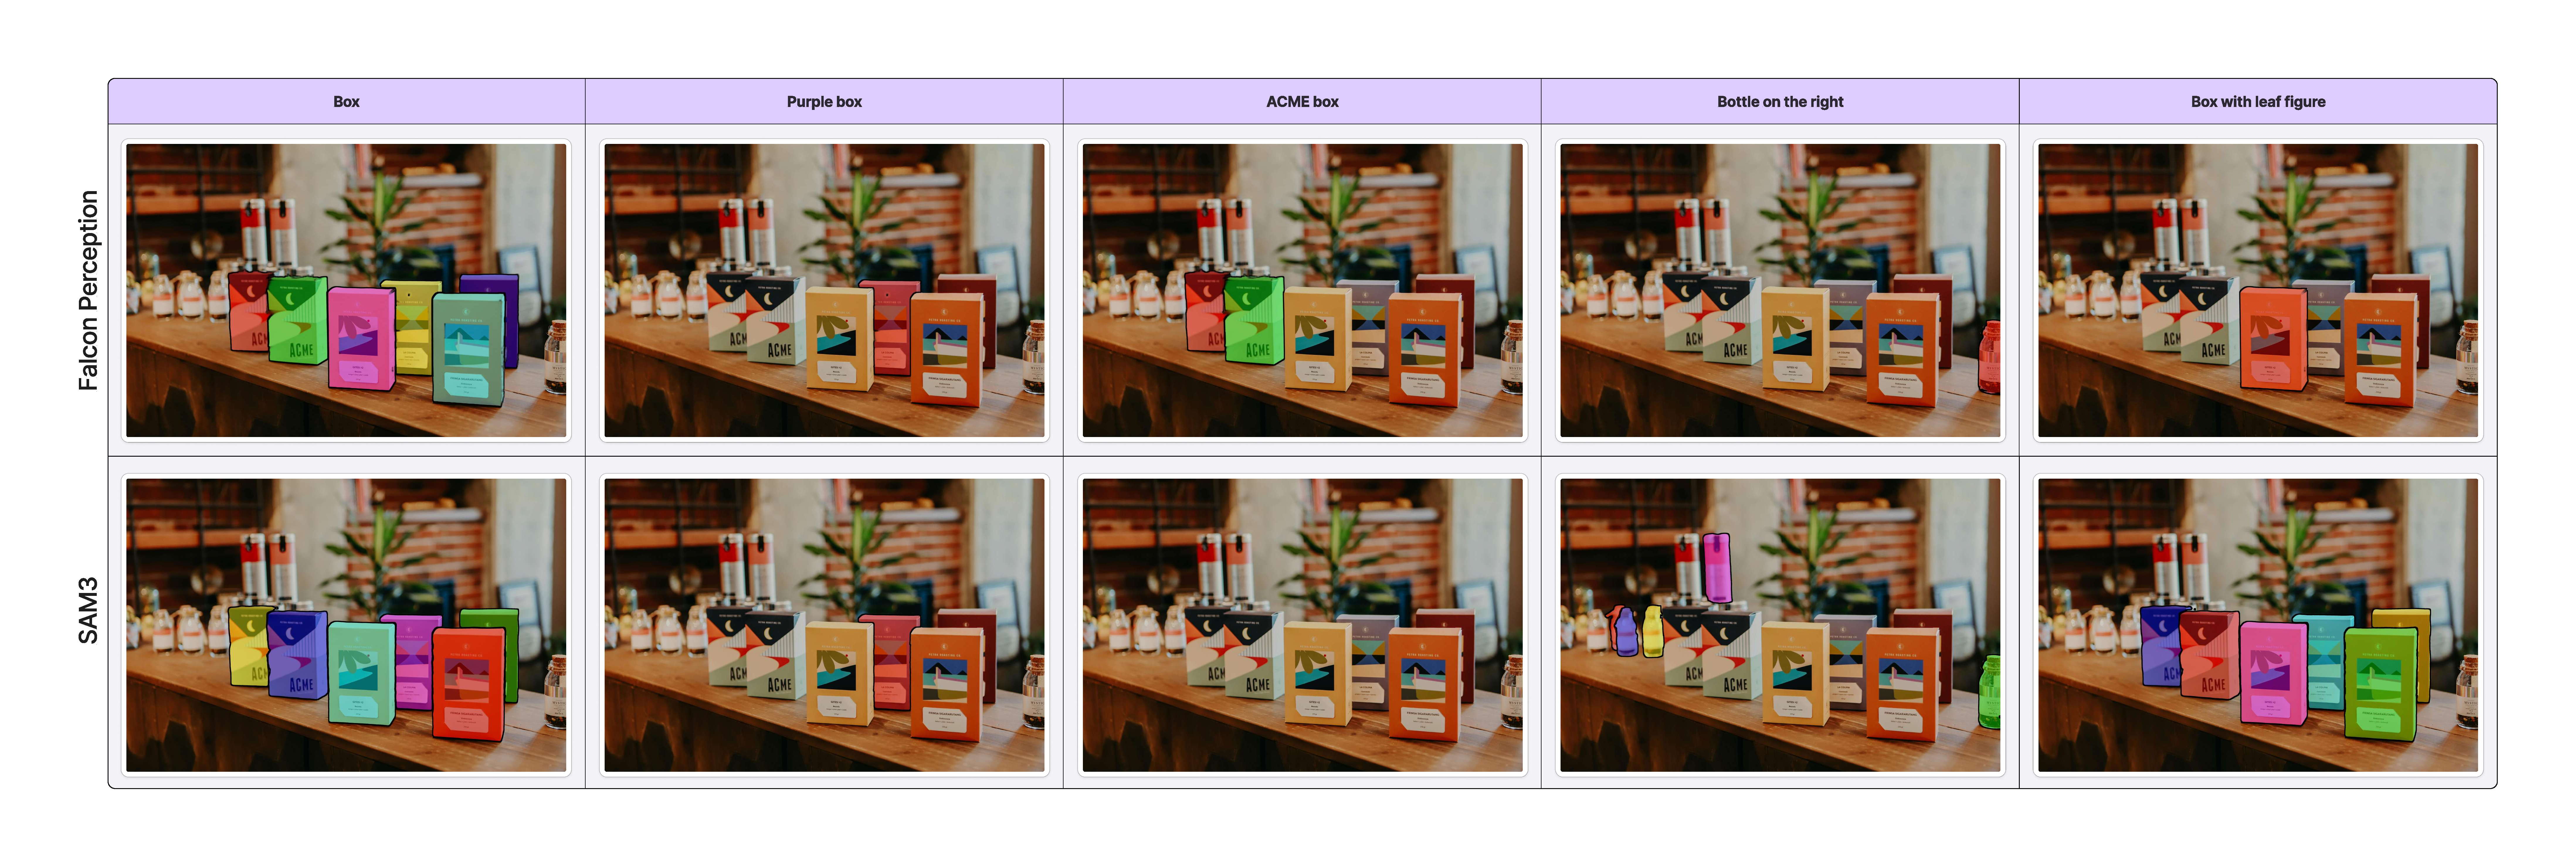
\includegraphics[width=1.0\textwidth, trim=4.5cm 4.5cm 4.5cm 4.5cm, clip]{figures/level_progression.pdf}
\caption{\textbf{Prompt progression across complexity levels.} We keep the image fixed and vary the text prompt to isolate the capabilities targeted by Levels~0--4 (Table~\ref{tab:complexity_levels}). Each panel shows the predicted masks for the same scene under progressively more specific prompts: from generic object classes (Level~0, \eg ``box''), to attribute binding (Level~1, \eg ``purple box''), to OCR-based identification (Level~2, \eg ``ACME box''), and then spatial/layout constraints (Level~3, \eg ``bottle on the right'') and fine-grained relational descriptions (Level~4). Falcon Perception remains stable as prompts become more compositional and text-dependent, while SAM~3 starts to fail on OCR-driven queries and higher-level constraints, either returning no masks or segmenting visually plausible but semantically wrong instances.}
\label{fig:levels_progression}
\end{figure}


Before diving into the training dynamics, we work on measuring progress for referring expression segmentation. Current benchmarks, such as RefCOCO, RefCOCO+~\citep{yu2016modeling}, and G-Ref~\citep{kazemzadeh2014referitgame}, have been important driving progress in the field. However, they suffer from two critical limitations. First, performance saturation: state-of-the-art models now routinely achieve $>80 \%$ acuracy, making it difficult to rank models. Second, and more importantly, they lack \textit{semantic granularity}. A \textit{hard} sample in these datasets conflates various challenges: complex prompt, spatial ambiguity, or world knowledge into a single metric. A model might fail because it cannot detect small objects, or because it does not understand a complex expression, but the benchmark score provides no signal to differentiate these failure modes.

\noindent To rigorously evaluate Falcon Perception and understand its capabilities, we introduce a hierarchical evaluation benchmark. Designed to disentangle the capabilities required for open-vocabulary segmentation, organizing samples into five distinct levels of complexity. This allows us to track capabilities progress effectively. 

\subsection{Complexity Levels}
\label{sec:complexity-levels}

Each sample is assigned a \emph{single} level label by construction, and prompts are intentionally written to target one dominant capability while avoiding cross-level cues (\eg, OCR prompts avoid spatial qualifiers such as ``left/right'', and spatial prompts avoid in-image text disambiguators). This yields a capability profile rather than a single scalar score. Please refer to Table \ref{tab:complexity_levels} for the levels definition and examples.


\begin{table}[t]
\centering
\footnotesize
\caption{Complexity-level taxonomy for our internal referring expression segmentation benchmark. Each sample is assigned a single level label by construction, enabling per-level capability profiling rather than a saturated aggregate score.\vspace{-0.3cm}}
\label{tab:complexity_levels}
\setlength{\tabcolsep}{5pt}
\renewcommand{\arraystretch}{1.2}
\begin{tabularx}{\textwidth}{p{0.05\textwidth} p{0.20\textwidth} >{\raggedright\arraybackslash}X p{0.21\textwidth}}
\toprule
\textbf{Level} & \textbf{Primary capability} & \textbf{Prompt ingredients \newline(single-skill by construction)} & \textbf{Examples} \\
\midrule
0 & General object classes &
\textbf{Rules:} whole objects only; machine-detectable categories; bbox-drawable; clear boundaries; no abstract concepts. &
\texttt{car}\newline\texttt{person}\newline\texttt{tree} \\
\midrule
1 & Fine-grained \newline attributes \& subtypes &
\textbf{Attributes:} color; size; shape; material.\newline
\textbf{State:} old/new; clean/dirty; broken/cracked; worn/well-maintained.\newline
\textbf{Subtype:} sedan/SUV/pickup; oak/palm/rose; tabby/golden retriever.\newline
\textbf{Functional:} open/closed; on/off; active/inactive.\newline
\textbf{Components:} sunglasses; cracked windshield; neon sign; petals. &
\texttt{red car}\newline\newline\texttt{broken fence}\newline\newline\texttt{open door} \\
\midrule
2 & Text as identifier (OCR) &
\textbf{Brand/product:} Coca-Cola; Nike; iPhone.\newline
\textbf{Variant:} Diet vs Regular; gluten-free vs regular.\newline
\textbf{Store/location:} Starbucks; McDonald's; Barnes \& Noble.\newline
\textbf{Signage/tags:} sale tag; prescription label; emergency exit. &
\texttt{Diet Coke bottle}\newline\newline\texttt{Nike shoes}\newline\newline\texttt{Emergency exit door} \\
\midrule
3 & Spatial relationships \& layout &
\textbf{Relative:} left/right/behind; above/below.\newline
\textbf{Depth:} foreground/middleground/background.\newline
\textbf{Ordering:} first/third/last (\eg, third from left).\newline
\textbf{Grouping:} in a row/line.\newline
\textbf{Containment:} inside/outside; boundary interactions. &
\texttt{car on the left}\newline\newline\texttt{third window from left}\newline\newline\texttt{person in the foreground} \\
\midrule
4 & Relationships \& interactions &
\textbf{Actions:} holding; wearing; pulling.\newline
\textbf{Functional links:} key for door; charger for phone.\newline
\textbf{Comparisons:} tallest/smallest/most damaged.\newline
\textbf{Physical:} resting on; hanging on; attached to.\newline
\textbf{Groupings:} dining set; lock and key; tools for repair. &
\texttt{person holding umbrella}\newline\newline\texttt{car pulling trailer}\newline\newline\texttt{tallest building in the row} \\
\bottomrule
\vspace{-0.2cm}
\end{tabularx}
\end{table}

\noindent \textbf{How to interpret the levels:} The levels are not a subjective notion of ``difficulty''; rather, each level isolates a dominant capability. Level~0 and Level~1 primarily probe open-vocabulary recognition and attribute binding. Level~2 isolates OCR-aware disambiguation where in-image text is the deciding signal between near identical instances. Level~3 isolates spatial grounding and layout understanding, testing whether the model forms a coherent 2D scene map. Level~4 isolates relational grounding where the target is defined through interaction rather than appearance. We therefore report per-level performance in addition to an overall average, yielding a capability profile that reveals \emph{where} a model fails (\eg, collapsing at OCR or relations). As shown in Figure \ref{fig:levels_progression}, for the same image, the different prompts highlight different capabilities from simply asking about boxes, to attributing with a color, then using the text written to retrieve the correct ones, followed by using spatial instructions, and finally using a finegrained description.\\

\subsection{Crowdedness and Long-Context Stress Test}
\label{sec:dense_stress}

In addition to semantic separation (Levels 0-4), we evaluate on \emph{dense} image with many instance per prompt. Crowded scenes stress long-context generation because the model must emit a long sequence of object queries and masks, maintain a stable ``object not found'' prior, and avoid duplication and drift as the number of instances $K$ increases. This regime is poorly characterized by existing referring benchmarks, which typically contain relatively few instances per image. We therefore report performance as a function of $K$ (\eg, $K \le 150$ in-distribution, and long-context settings up to $K \approx 600$). This isolates whether a model fails due to semantic understanding (captured by the complexity levels) or due to long-context dynamics (crowdedness), and directly measures the stability of our autoregressive Chain-of-Perception interface in dense environments. It is worth mentioning that this category still register under Level~-1 with simple nouns, and the complexity comes from the instance count.

\subsection{Creation and Statistics}
\label{sec:benchmark_construction}

\noindent \textbf{Construction:} The benchmark was created internally by team members who contributed to training Falcon Perception. Prompts and target masks were curated with domain expertise to ensure both high quality and clean semantic separation across the complexity levels. In particular, each sample is assigned a \emph{single} level label by construction: prompts are written to isolate one dominant capability (\eg, OCR disambiguation without spatial cues), enabling diagnostic evaluation rather than conflating multiple failure modes. In addition, we curate a separate crowdedness subset to stress long-context generation and dense instance segmentation.

\noindent \textbf{Size:} The benchmark contains approximately $\sim$5k samples  across Levels~0--4, and an additional $\sim$400 samples dedicated to crowdedness stress testing.
